\documentclass[a4paper,12pt]{report}
\usepackage[T1]{fontenc}
\usepackage[utf8]{inputenc}
%\usepackage[shorthands=off,english,ngerman]{babel}
% uncomment to use german without "" being interpreted as umlauts
\usepackage[english]{babel}
\usepackage[sfdefault]{roboto}
\usepackage[margin=1in]{geometry}
\usepackage{amsmath}
\usepackage{amsfonts}
\usepackage{amssymb}
\usepackage{amsthm}
\usepackage{graphicx}
\usepackage{subcaption}
\usepackage{color}
\usepackage{xcolor}
\usepackage{url}
\usepackage{textcomp}
\usepackage{parskip}
\usepackage[numbers]{natbib}
\bibliographystyle{plainnat}
\usepackage{hyperref}[xcolor]
\definecolor{cite-color}{HTML}{ff81ff}
\definecolor{url-color}{HTML}{d094d0}
\definecolor{link-color}{HTML}{2d212d}
\hypersetup{
    colorlinks=true,
    urlcolor=url-color,
    linkcolor=link-color,
    citecolor=cite-color,
}

\usepackage{epigraph}
\usepackage{soul}
\usepackage{wrapfig}
\usepackage[dvipsnames]{xcolor}
\usepackage{listings}

\lstdefinelanguage{Kotlin}{
  comment=[l]{//},
  commentstyle={\color{gray}\ttfamily},
  emph={filter, first, firstOrNull, forEach, lazy, map, mapNotNull, println},
  emphstyle={\color{OrangeRed}},
  identifierstyle=\color{black},
  keywords={!in, !is, abstract, actual, annotation, as, as?, break, by, catch, class, companion, const, constructor, continue, crossinline, data, delegate, do, dynamic, else, enum, expect, external, false, field, file, final, finally, for, fun, get, if, import, in, infix, init, inline, inner, interface, internal, is, lateinit, noinline, null, object, open, operator, out, override, package, param, private, property, protected, public, receiver, reified, return, return@, sealed, set, setparam, super, suspend, tailrec, this, throw, true, try, typealias, typeof, val, var, vararg, when, where, while, SegmentedButton},
  keywordstyle={\color{NavyBlue}\bfseries},
  escapeinside={//(`}{`)},
  morecomment=[s]{/*}{*/},
  morestring=[b]",
  morestring=[s]{"""*}{*"""},
  ndkeywords={@Composable, @Preview, @Deprecated, @JvmField, @JvmName, @JvmOverloads, @JvmStatic, @JvmSynthetic, Array, Byte, Double, Float, Int, Integer, Iterable, Long, Runnable, Short, String, Any, Unit, Nothing, },
  ndkeywordstyle={\color{BurntOrange}\bfseries},
  sensitive=true,
  stringstyle={\color{ForestGreen}\ttfamily},
}
\lstset{
  breaklines=true,
  breakatwhitespace=false,
  columns=fullflexible,
  showspaces=false,  % REMOVES SPACES FROM HTML CODE, DO NOT EDIT
  showtabs=false,
  showstringspaces=false, % REMOVES SPACES FROM HTML CODE, DO NOT EDIT
  keepspaces=true         
}

\title{Creating an "AndroidToolbox" App \& Desktop Insecurity}
\author{[redacted]}
\date{\today}

\begin{document}
\begin{titlepage}
    \centering
    {\Huge\bfseries Creating an "Android Toolbox" App \& Desktop Insecurity\par}
    \vspace{1cm}
    {\LARGE Maturaarbeit \par}
    {\Large \textsc{[redacted]}\par}
    \vspace{1cm}
    {\Large [redacted]\par}
    {\Large Betreuungsperson: [redacted] \par}
    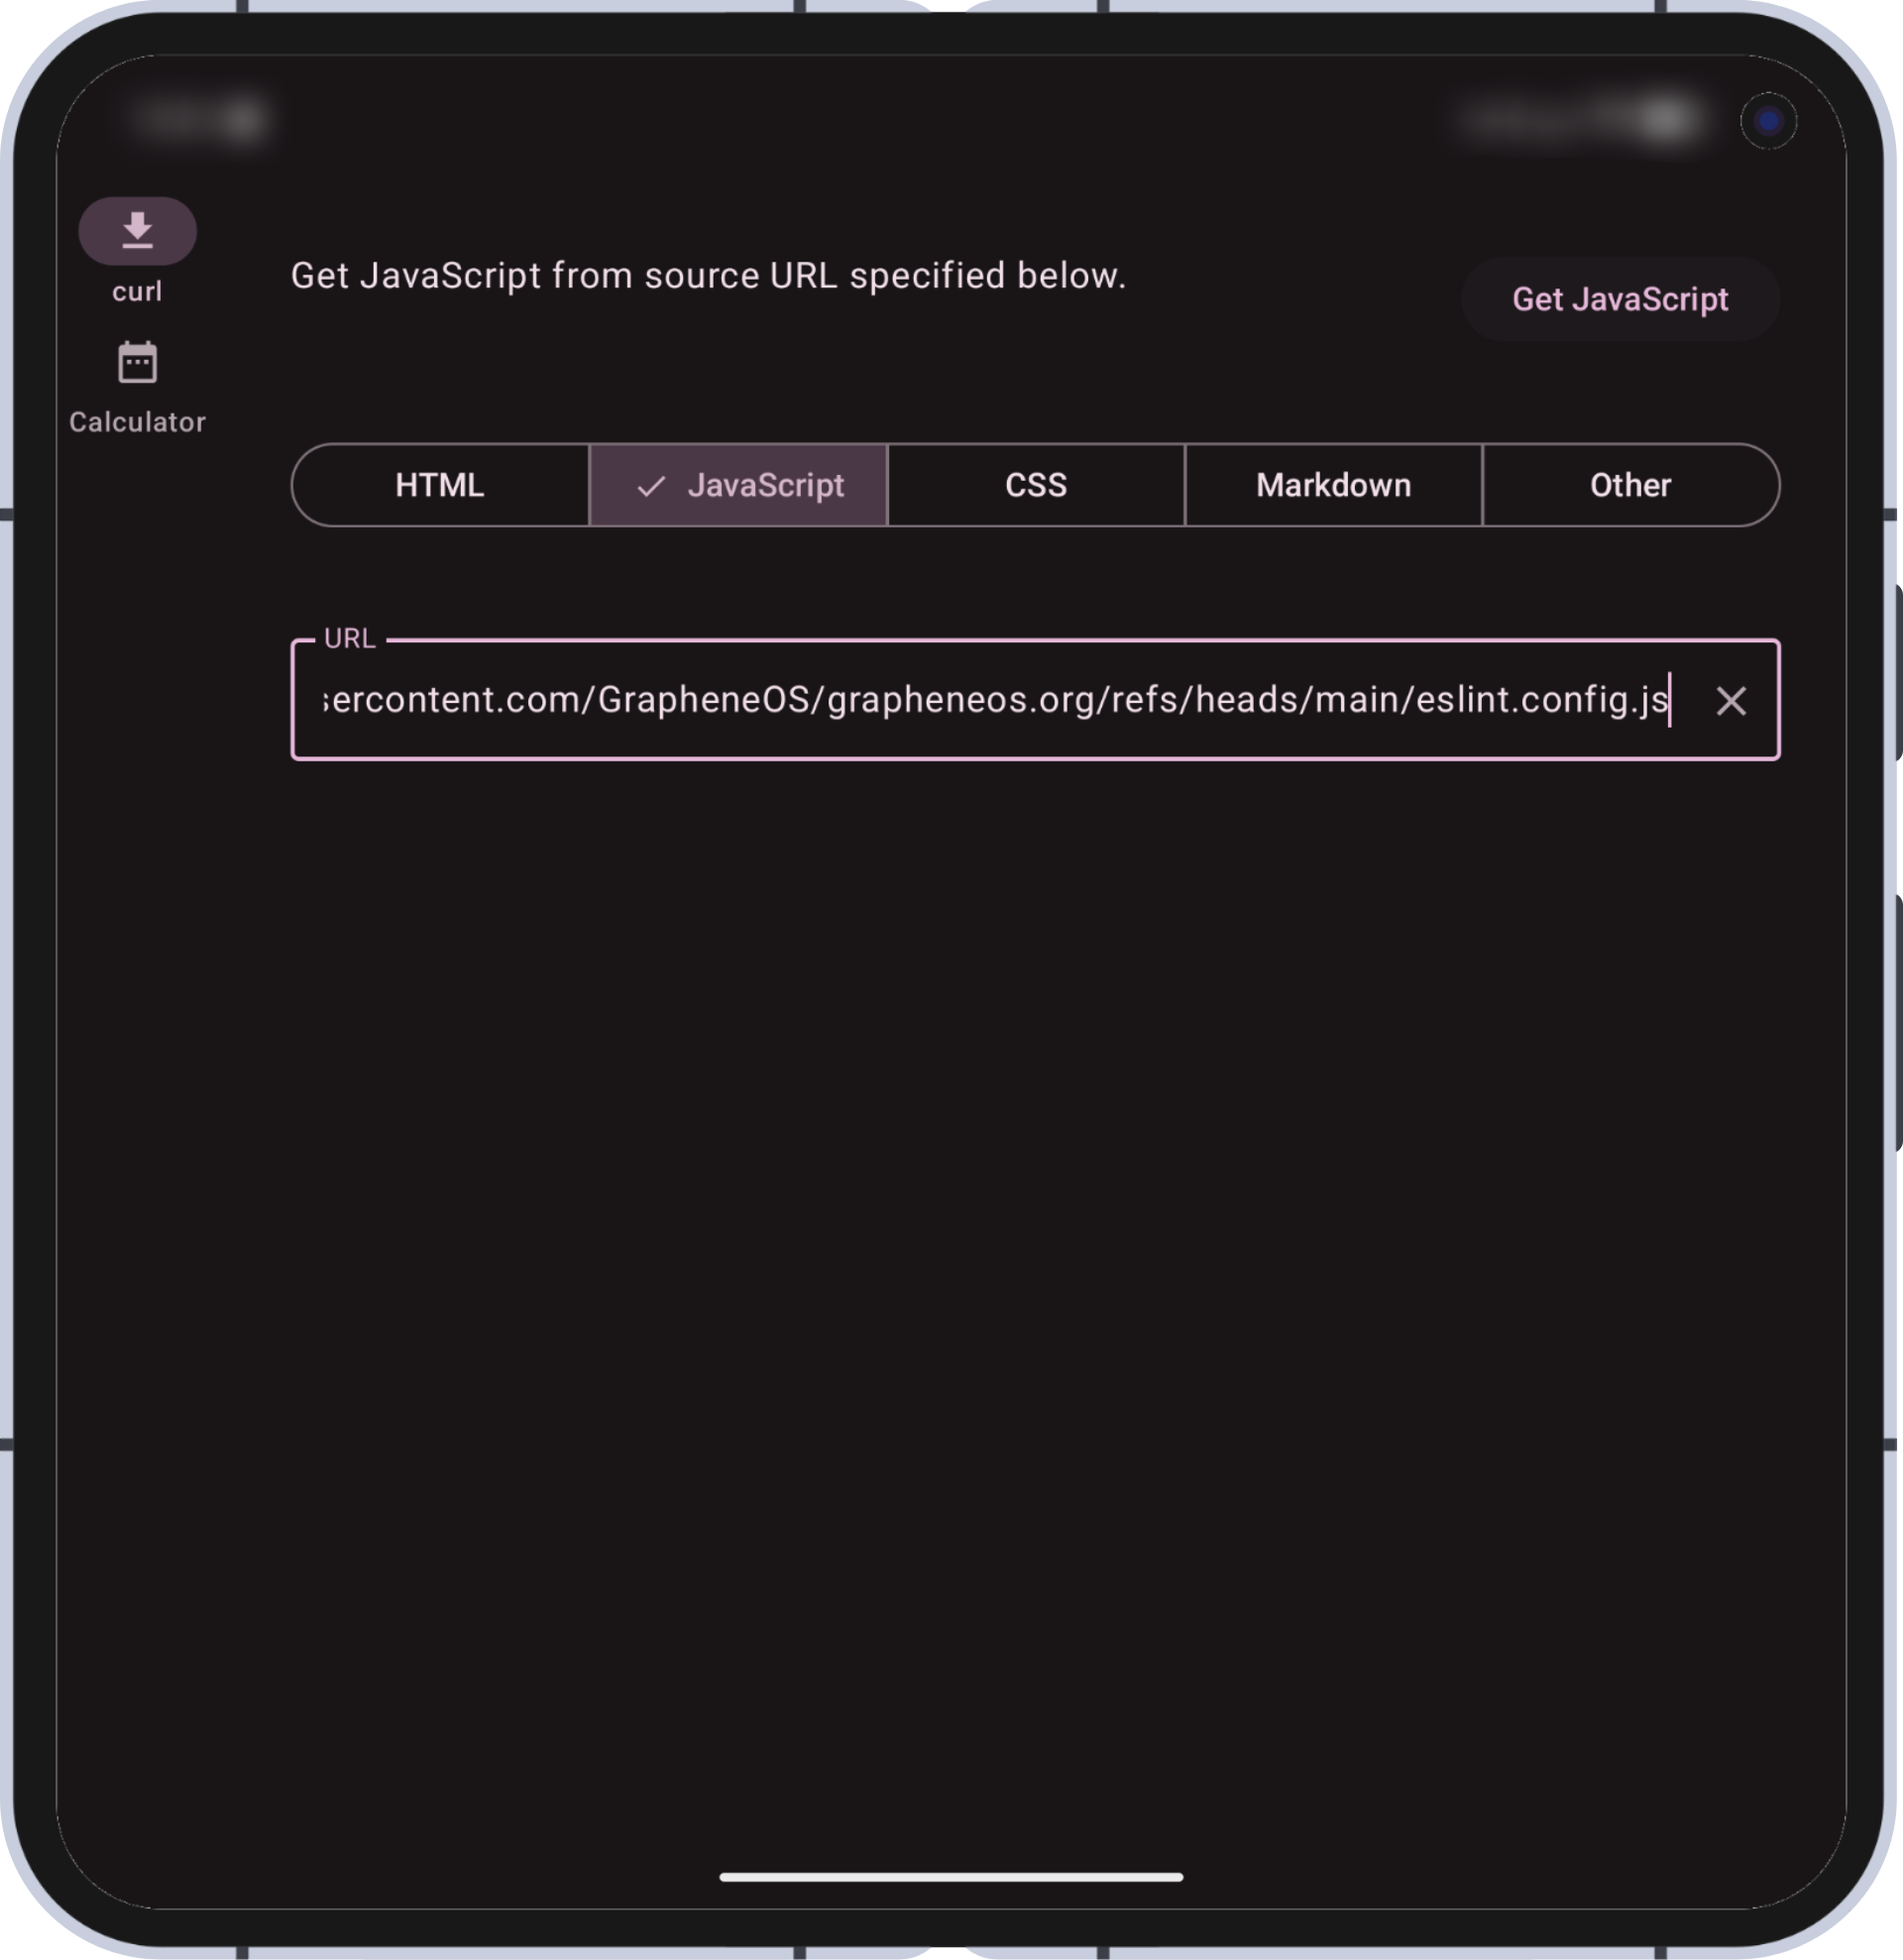
\includegraphics[width=0.9\linewidth]{app_screenshot-pixel10profold.png} \\
    {\footnotesize Screenshot, image modified from \cite{pixel10fold}}
    \vfill
    {\large \today\par}
\end{titlepage}

\begin{abstract}
There is a common misconception that so-called "Desktop" operating systems, usually running on x86 \textsuperscript{\citep{x86}} hardware are more secure than "Mobile" ones, which usually are designed for ARM \textsuperscript{\citep{arm}} SoCs. Contrary to this common misconception, desktop operating systems are in fact commonly far less secure both in terms of hardware, as well as software security. This paper aims to clarify those common misconceptions and explain the motivation behind creating an application (App) that expands functionality which the author of this paper considers to be critically missing and therefore fixes the issue of insecure operating systems by making them unnecessary for a certain demographic of users that wish to prioritize security over other aspects in a landscape of constantly evolving threats.
\end{abstract}
\tableofcontents

\chapter{Preface}
This paper originates from what the author of this paper believes to be a critical need to address the fundamental insecurities inherent in modern computing environments. The author wished to resolve these issues by developing a secure operating system from the ground up based on a microkernel architecture, or by modifying an existing base deemed fit for purpose. However, the practical requirements for such an undertaking proved prohibitive and unrealistic. The hardware resources alone that are necessary to compile a modern operating system, specifically the high-core-count CPUs and extensive memory required for AOSP, are beyond the author's current financial and technical reach. Additionally, the author recognizes that a lack of formal university training in computer science and decades of professional software development experience makes the creation of a kernel-level replacement an unrealistic goal for them.

Through a study of hardware and software architectures and their passion and personal interest for cybersecurity and privacy, the author identified a prevailing misconception that desktop operating systems are more secure than mobile ones. As the author claims, in reality, x86 hardware is constrained by technical debt and backwards compatibility, which prevents the implementation of advanced protections such as hardware memory tagging. ARM-based systems, and specifically distributions like GrapheneOS, provide a more secure foundation by implementing a verification chain from a hardware root of trust to the userspace, making it possible for the end user to trust both the OS and userspace applications running on it, if trust in the developers of both is assumed.

While GrapheneOS offers significant attack surface reduction, the author identified a lack of specific functionality necessary for certain users, including themselves. Because the creation of a new operating system was not feasible by them, the author focused on developing an application that expands the capabilities of an existing secure platform. This application was built with a strict adherence to security best practices, including the use of synchronous MTE and AOT compilation for example. This paper documents the security justifications for this approach and explains the technical motivation behind the resulting software. It also hopes to provide insight into the process of developing a secure application and wishes to inspire others to do the same. 

Unless otherwise noted, this work, including the author's original text and images, is dedicated to the public domain under \href{https://creativecommons.org/publicdomain/zero/1.0/}{CC0 1.0 Universal}.

\chapter{Introduction}
\section{Motivation}
There is a common misconception that so-called "Desktop" operating systems, usually running on x86 \textsuperscript{\citep{x86}} hardware, are more secure than "Mobile" ones designed for ARM \textsuperscript{\citep{arm}} SoCs. This couldn't be further from the truth. In fact, desktop systems are commonly far less secure in terms of both hardware and software. A major part of this problem is that x86 hardware is limited by technical debt and backwards compatibility requirements. As will be discussed in the Hardware Security section, this makes it impossible to implement advanced features like hardware memory tagging (MTE) which are available on ARM-based SoCs.

The software side is also very problematic because of the reliance on monolithic kernels. These kernels create a large attack surface that is difficult to defend. While microkernels provide better process isolation and solve the confused deputy problem, they are not widely used. This structural weakness is now a critical issue due to the rise of AI-based tools. These tools allow remote attackers to automate the discovery of vulnerabilities and create exploit chains much faster than a human can. As the author explains in the \hyperref[google-failure]{failures to defend section}, even multi-billion-dollar corporations like Google have been overwhelmed by the volume of AI-discovered vulnerabilities, which has resulted in critical security patches being delayed by weeks or months.

The author would ideally like to solve these issues by creating a secure operating system from scratch using a microkernel. However, this is not possible due to the limitations described in detail in the Limitations section. Compiling AOSP requires hardware and financial resources that the author does not have, such as 32-core, or ideally 64-core CPUs and massive amounts of storage and RAM. Additionally, the author lacks the decades of professional software developer experience required to replace a kernel like Linux and high-level computer science education like a bachelor in computer science at a respected university.

Therefore, the author of this paper concludes that the most realistic solution is to use an existing, reasonably secure OS that implements a verification chain from a hardware root of trust (RoT) to the userspace. A Google Pixel smartphone running \citeauthor{grapheneos} is ideal for this because it provides meaningful attack surface reduction and avoids many of the security regressions found in standard Android\texttrademark \textsuperscript{\citep{android-tm}} distributions or \hyperref[aosp]{AOSP} forks.

Despite these advantages, the author considers certain functionality to be critically missing from \hyperref[aosp]{AOSP}-based distributions. This paper aims to clarify the aforementioned security misconceptions and explain the motivation behind creating an application (App) that provides this missing functionality. By doing so, the author aims to make insecure operating systems unnecessary for a specific demographic of users who prioritize security over other aspects in a landscape of constantly evolving threats.

\subsection{Limitations}
This paper is also limited by the resources, which tha author can dedicate to it. While the author would like to create a secure operating system (OS) from scratch or modify an existing one to meet the author's security standards, this would require significant time and monetary effort. Even during the creation of this App, the author frequently encountered limitations in the form of their laptop running out of memory to compile the app and/or compilation taking a significant amount of time. 
In order to compile \hyperref[aosp]{AOSP} for example, the author of this paper would need a computer that has at minimum four times as much storage as their current laptop at time of writing has and ideally at least a CPU with 32 cores. This would be a computer costing multiple thousands of swiss francs that will require significant amount of power to operate, likely tripping the circuit breaker if run from an outlet in the author's home. 
The author would also like to point out that even multi-billion-dollar market cap corporations like Google have failed at for example replacing the Linux\textsuperscript{\citep{linux}}kernel, which is a \hyperref[monokernel]{monolithic kernel} used in \hyperref[aosp]{AOSP} and \hyperref[aosp]{AOSP}-based distributions with a \hyperref[microkernel]{microkernel}.
In addition to limitations completely outside the author's control, the author would also like to acknowledge they are limited by their skills and knowledge. While they have spent many hours researching, planning and studying for this project to the best of their ability, they are unable to make up for a lack of decades of software developer experience and a university degree in computer science. 

\section{Cybersecurity}
\subsection{Definitions}
Before examining different aspects of mobile and desktop OS security, it's necessary to first define what certain terms mean, and provide an explanation of some complex topics.
\subsubsection{Hardware}
The physical device(s), e.g. the phone, laptop or other form of computer.

\subsubsection{Firmware}
This encompasses the low-level code that serves as an interface between the software and hardware of a system. This can be the kernel of an OS or Hardware Access Layer (HAL) APIs. Device drivers such as the display driver, audio driver, etc are firmware. Firmware can be part of a kernel or run in userspace.

\subsubsection{Kernel}
There are three common structures of an OS kernel, either a  monolithic kernel\textsuperscript{\ref{monokernel}}, which is more common a hybrid kernel\textsuperscript{\ref{hybridkernel}}, or a microkernel\textsuperscript{\ref{microkernel}}. Further detailed information is provided in the \hyperref[arches]{architectures} section.
\subsubsection{Userspace}
The userspace is the unprivileged layer in which user applications run. For example: web browsers\textsuperscript{\hyperref[browsers-note]{*}}, text editors, media players, etc.

\textbf{Note:}\\
\label{browsers-note}
This is not entirely true, since browsers often might require privileged user namespaces\textsuperscript{\citep{userns}} in order to properly utilize their sandbox. This has been an issue for security-focused Linux operating systems like \citeauthor{secureblue}, the developers of which have had to consider the trade-offs between different approaches, leading to them publishing an article on their website about it.\textsuperscript{\citep{secureblue-userns}} The author of this paper agrees with this approach and have contributed to similar discussions on websites dedicated to correcting misinformation and debunking myths. An archive of some of this work is available on an statis page hosted by someone the author of this paper knows personally.\textsuperscript{\citep{security-advice}} The author doesn't endorse the current contents of this archive however, since it has not been updated and does not fully reflect the current state of cybersecurity both in terms of defense and offense, which are shaped by evolving threat actors utilizing AI-based tools. This archive only serves to preserve information that might otherwise be lost. 

\subsection{Attackers}
\subsubsection{Types of attackers}
There are multiple types of attackers a secure system has to sufficiently protect against.
\begin{itemize}
    \item Local attackers with physical access to the device
    \item Local attackers without physical access to the device
    \item Remote attackers (Internet)
\end{itemize}
\subsubsection{Evolving threat actors}
Recently it has also become crucial to protect against automatic exploitation by AI-based or assisted tools, which allow remote attackers to automate targeted exploitation en masse. This has resulted in a large quantity of so called "phishing" attacks that use personal information and AI to trick the user into compromising their device. Additionally, AI-based tools can attempt to exploit a piece of software many times without having to take breaks several orders of magnitude faster than a human can, resulting in a vast surge of new vulnerability discoveries. Coupled with newer AI models being able to chain together exploits in order to form a so-called "exploit chain", which usually requires a skilled human or team of humans working for weeks or even months to create, the amount of malware has drastically increased and defensive measures are more important than even before. 
\subsubsection{Failures to defend}
\label{google-failure}
The author would also like to point out that the surge of AI-based vulnerability discoveries has and still is actively impacting how Android\texttrademark \textsuperscript{\citep{android-tm}} security patches are handled. For example, \citeauthor{grapheneos} has reported in multiple, consecutive posts that Google has been overwhelmed by the large volume of vulnerabilities found by AI models, resulting in a situation where the full set of high and, more importantly, critical severity patches are now only available through the latest yearly and QPR2 releases, with only a subset deemed an imminent risk being backported to older security-supported releases. This means patches are delayed by weeks or even months, even though some of these patches are for vulnerabilites which are being widely exploited.
Furthermore, while Android OEMs are granted early access to security bulletin patches, a system \citeauthor{grapheneos} disagrees with, but utilizes to ship patches before they are publicly available, which benefits their project massively. They do not actually utilize the capability granted to them and ship the patches even later than Google to their modified verions of Android\texttrademark \textsuperscript{\citep{android-tm}}, further degrading security for end users, while the amount of known (and unknown) vulnerabilities increases over time.\textsuperscript{\citep{grapheneos1,grapheneos2,grapheneos3}}
\citeauthor{grapheneos} provides a list of patches for which a CVE (common vulnerability and exposure) has been assigned to with each security preview release they publish. As of writing, the latest release, 2026100600 has a total of 122 additional CVEs listed, 8 of them being marked as critical. All of those 122 CVEs are currently, as of writing, unpatched for the majority of Android\texttrademark \textsuperscript{\citep{android-tm}} users. This does not include vulnerabilities that are not assigned a CVE.
Attackers however can trivially reverse-engineer the patches and thus the majority of those vulnerabilities become widely known and exploited by malicious threat actors like criminals, stalkers and nation-state-actors for the goal of targeted attacks or mass exploitation for financial or other gains. Security by obscurity does not work and it should always be assumed that attackers have encyclopedic knowledge of known vulnerabilities present in any software relied upon, in addtion to yet unkown (0day) exploits.

\subsection{Architectures}
\label{arches}
Operating systems are often categorized by their kernel structure, since the kernel represents the most important part of the OS and also serves as a good indicator of the security and compatibility of an OS in terms of already existing software. Therefore, it is crucial to understand how these different types of kernels are structured and where they are used before making a decision on whether an OS can be sufficiently secured against modern attackers, be they local or remote, which utilize advanced hacking tools like AI-based exploit scanning and/or automation.

\parbox[t]{\textwidth}{
  \subsubsection{Monolithic Kernel}
  \label{monokernel}
  \begin{wrapfigure}{l}{0.45\textwidth} 
      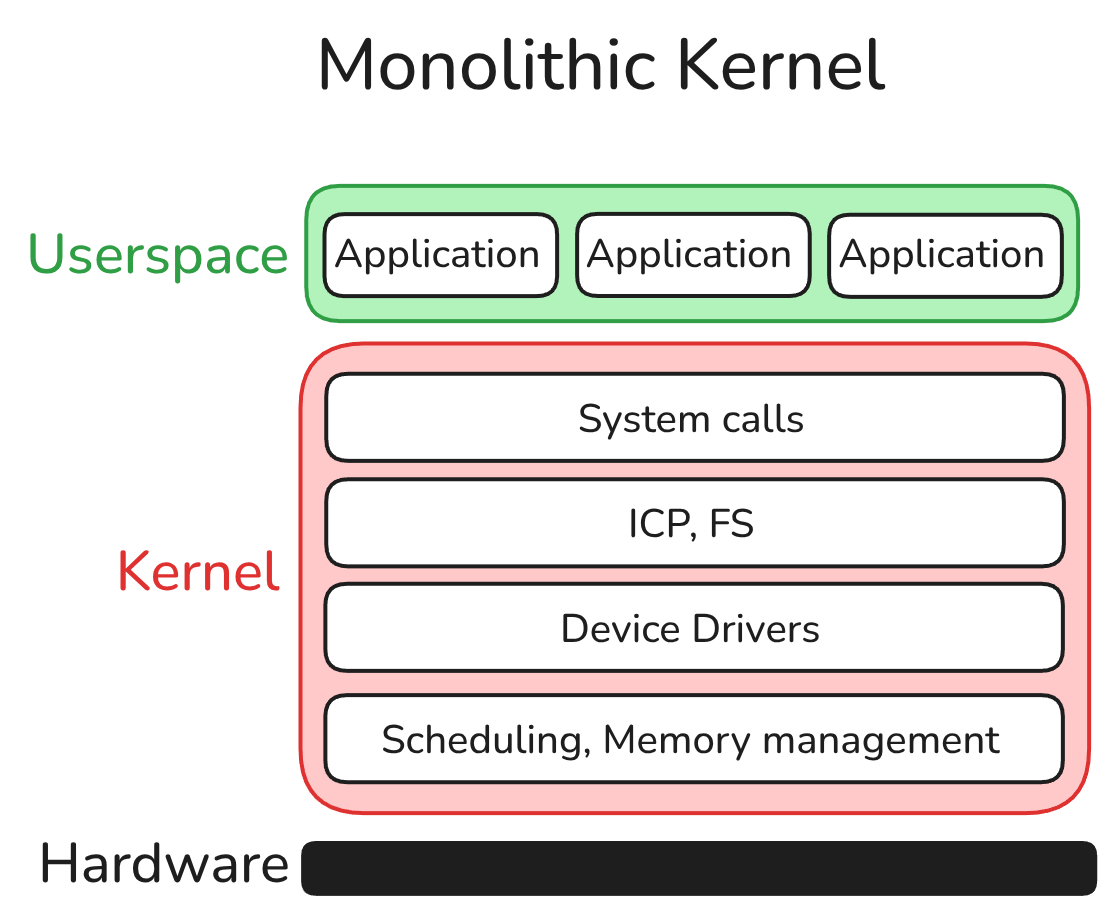
\includegraphics[width=0.9\linewidth]{monolithic-kernel.png}
      \caption{Monolithic Kernel \citep{monokernel-graph}}
  \end{wrapfigure}
  A monolithic kernel is essentially one large program that handles drivers, IPC, Memory allocation, etc. They are the most common, since the Kernel running on most Systems running all the Servers in the world run Linux\textsuperscript{\citep{linux}}, a UNIX-like\textsuperscript{\citep{unix}} Kernel developed originally by Linus Torvalds, based on Unix\textsuperscript{\citep{unix-og}}. Monolithic kernels are the most common structure used in Operating Systems due to their relative simplicity to implement and existing software written for them. They are lacking in terms of security as compared to Hybrid and Microkernels due to their nature as a Monolithic structure, lacking in intra-kernel process isolation and being more difficult to pentest and debug. In recent years, there have been many attempts at improving Kernel security by implementing features such as Hardware Memory Tagging (MTE), which is used by Apple Inc. and \citeauthor{grapheneos}. \textsuperscript{\citep{mte-gos} \citep{apple-mte}}
}


  \subsubsection{Microkernel}
  \label{microkernel}
  \begin{wrapfigure}{l}{0.45\textwidth} 
      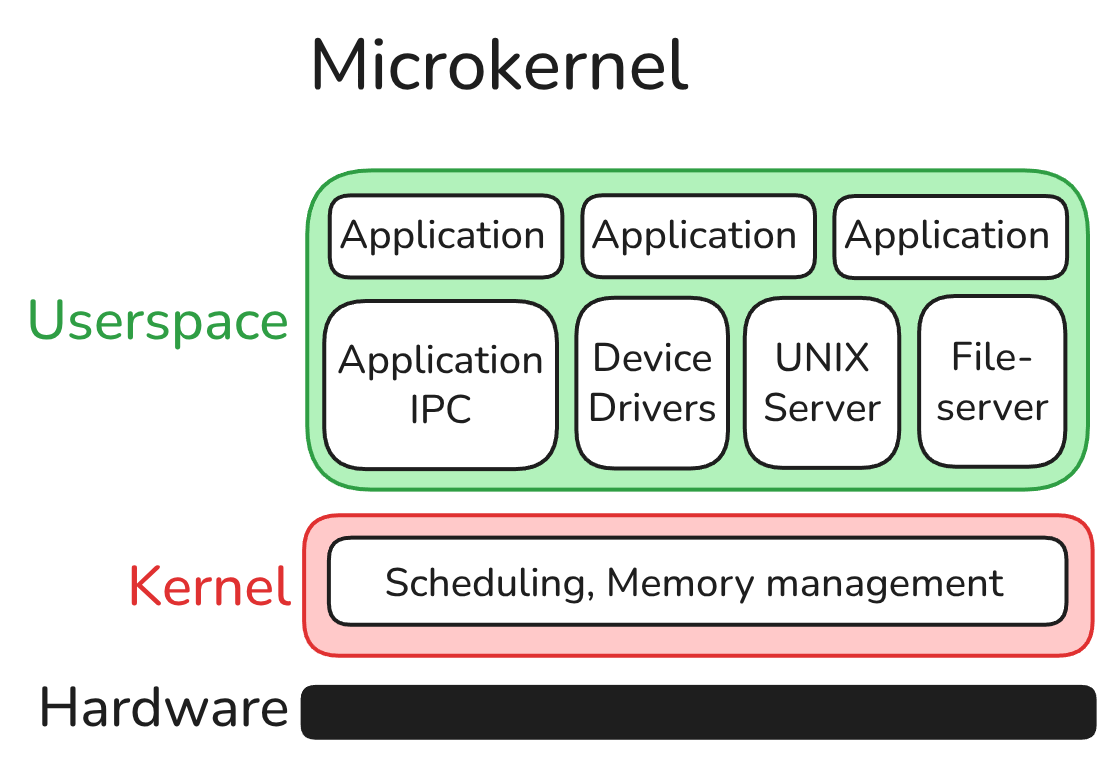
\includegraphics[width=0.9\linewidth]{microkernel.png}
      \caption{Microkernel \citep{microkernel-graph}}
  \end{wrapfigure}
  Microkernels, as the name suggests, consist of minimal kernel-space processes. Any process that can be run in userspace is run in userspace. Only the most essential components, such as system calls, process separation, resource management, or IPC (Inter-Process-Communication), are delegated to the kernel. Drivers run in userspace. The function of a microkernel is only to provide a medium for communication with each other and separation of processes. This makes microkernel designs are more stable, as they are easier to debug and test, and buggy drivers cannot cause kernel panics, unlike with monolithic kernel systems. More importantly, microkernels are far more secure since different processes are sandboxed and isolated from each other, providing excellent intra-kernel isolation. This is especially true for systems based on capability and not identity. Capability-based security\textsuperscript{\citep{capability-based-sec}} refers to treating a process by its capability and not access granted based on identity. For example: if a process maliciously acquires access to confidential data it should not, said process itself will also become confidential. This solves the famous confused deputy problem\textsuperscript{\citep{conf-dep}}, originally covered by Norm Hardy in his 1988 Paper \citetext{The\ Confused\ Deputy:\ (or\ why\ capabilities\ might\ have\ been\ invented)}\textsuperscript{\citep{conf-dep-original}}.
\parbox[t]{\textwidth}{
  Examples of microkernel OSs with capability-based security are \citeauthor{redox} or \citeauthor{fuchsia}. Other examples that don't utilize capabilities on a foundational level are HarmonyOS\textsuperscript{\citep{harmonyos}} and its base, OpenHarmony\textsuperscript{\citep{openharmony}}, which in turn is a hard fork of \hyperref[aosp]{AOSP}. The author of this paper has previously suggested in direct messages to the developers of \citeauthor{grapheneos} that OpenHarmony could potentially be used as a replacement for the Linux kernel, which is a long-term goal of \citeauthor{grapheneos}. The developers pointed out that OpenHarmony has not been independently audited against its claims and diverges from the goals of \citeauthor{grapheneos}. It aims to create an integrated OS for iOT devices like smart TVs, smartwatches, etc to be used with a Huawei account, similarly to what is often referred to as the "Apple Ecosystem". This is also something that OpenHarmony itself states is a goal:
  \begin{quote}\textit{
      Distributed data management leverages DSoftBus to manage application data and user data distributed on different devices. Under such management, user data is no longer bound to a single physical device, and service logic is decoupled from storage. As your applications are running across devices, their data is seamlessly transmitted from one device to another, creating a foundation for a user experience that is smooth and consistent.}\textsuperscript{\citep{openharmony-docs-data_dist}}
  \end{quote}
}

\parbox[t]{\textwidth}{
  \subsubsection{Hybrid Kernel}
  \label{hybridkernel}
  \begin{wrapfigure}{l}{0.45\textwidth} 
      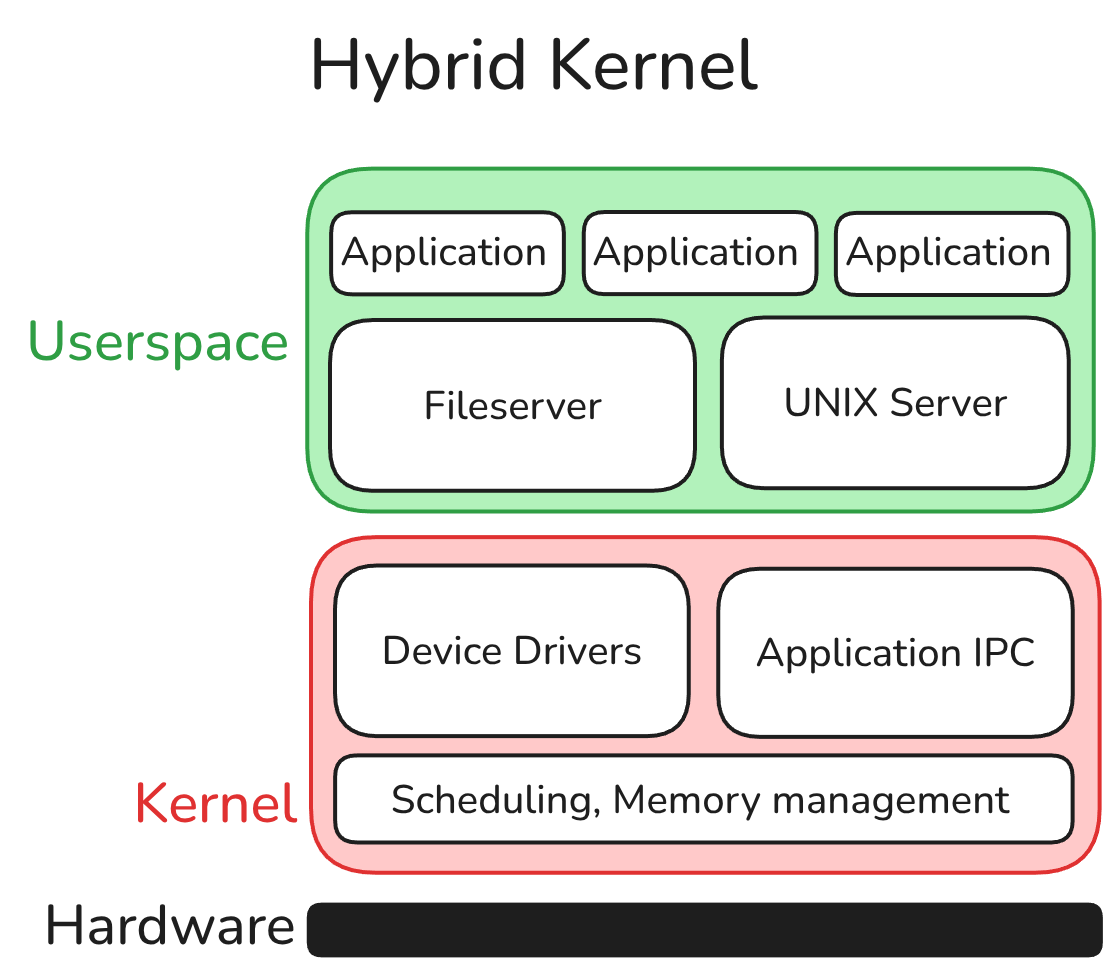
\includegraphics[width=0.9\linewidth]{hybrid-kernel.png}
      \caption{Hybrid Kernel \citep{hybridkernel-graph}}
  \end{wrapfigure}
  Hybrid kernels are usually former monolithic-kernel-based operating systems, that over time have processes transferred from the Kernel to the userspace. Examples of Hybrid kernels are the XNU kernel, which is the Open-Source basis of Apple Inc.'s operating systems such as macOS or iOS,\textsuperscript{\citep{xnu}} the NT kernel developed by Microsoft \textsuperscript{\citep{ntkernel}}, and Plan 9 from Bell Labs.\textsuperscript{\cite{plan9}} It should be noted however, that Microsoft Windows does not implement proper application sandboxing and userspace process isolation, giving any application almost full system access.
  Since \hyperref[aosp]{AOSP} is slowly moving a larger section of system processes into userspace and disabling more of the Linux kernel at build time, it might be classified as Hybrid Kernel at some point in the future as well. However, ideally it would be moved to a \hyperref[microkernel]{microkernel} architecture, since there are very few functions the Linux kernel is necessary for in \hyperref[aosp]{AOSP}.
}

\parbox[t]{\textwidth}{
\subsubsection{AOSP}
\label{aosp}
The following is the Architectural stack of AOSP. It's an example of a monolithic kernel based OS that does implement sufficient security protections, in part by delegating a large portion of important code into the unprivileged userspace, however it still uses the Linux\textsuperscript{\citep{linux}} Kernel with unnecessary features disabled for attack surface reduction. In \citeauthor{grapheneos}, as part of the project's many security enhancements, the Kernel is hardened as well.\textsuperscript{\citep{gos-mitigations}} Very few system services have root privileges on AOSP-based distributions, such as Android\texttrademark \textsuperscript{\citep{android-tm}} or \citeauthor{grapheneos}. The Hardware Access Layer (HAL) is also a major improvement that AOSP introduces. It acts as a bridge between the higher-level Android Framework and device drivers and provides modularity and security improvements. 

\parbox[t]{\textwidth}{
\begin{wrapfigure}{l}{0.45\textwidth}
    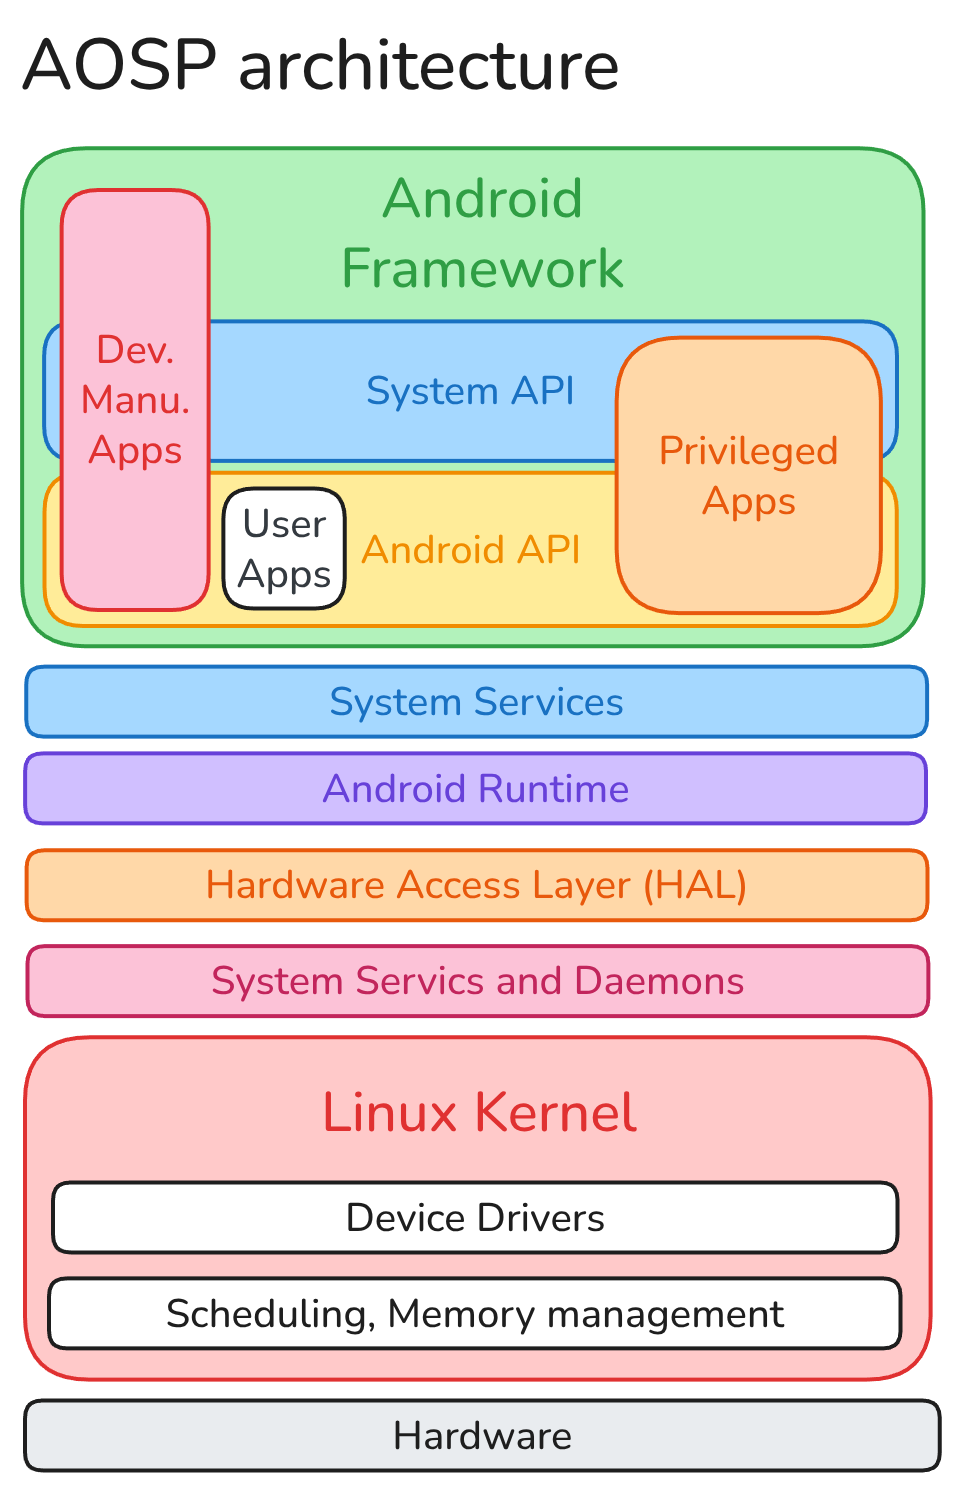
\includegraphics[width=0.9\linewidth]{android-stack.png}
    \caption{AOSP Architecture \cite{aosp-graph}}
\end{wrapfigure}
Contrary to \hyperref[aosp]{AOSP} and other AOSP-based distributions such as Android\texttrademark \textsuperscript{\citep{android-tm}} or the Googlebook OS (codenamed AluminiumOS\textsuperscript{\citep{aluminium-os}}), on \citeauthor{grapheneos} all apps are sandboxed equally, including Google Mobile Services (GMS), which can be installed unmodified from the OS-provided App store. GMS is treated as any third-party app and runs without special priviliges, the same is true for the system apps \citeauthor{grapheneos} ships with by default. The application sandbox is also further improved, network, clipboard access and sensors permissions can be revoked and over 45 different exploit protections on top of \hyperref[aosp]{AOSP} are introduced. \textsuperscript{\cite{exploit-protect-gos}} Most of these exploit protections are under-the-hood improvements with no UI for the user to customize them, but some that might cause incompatabilities can be customized OS-wide or per-app.
}
}

\newpage
\subsection{Hardware Security}
The most difficult problem to fix with the so-called "Desktop" operating system security is the problem of inadequate hardware security. While issues on the software level can be mitigated by an advanced user capable of configuring their system and implementing userspace application sandboxing and system process isolation, as well as even cryptographically verify the operating system itself, only hardware vendors can improve the security on a hardware level, but they are limited by backwards compatibility requirements and technical debt of outdated technology. 
x86 hardware security is lacking compared to ARM-based SoCs, which can implement advanced security features such as hardware memory tagging (MTE), while x86 hardware is limited to the very basic HSI \textsuperscript{\citep{hsi}} specification, but decades of software is written to use x86 instructions, so fundamentally changing the architecture proves impossible. To implement Verified Boot for Chromebooks and Googlebooks, Google mandates the use of an additional \citeauthor{opentitan}-based HSM called "Titan C/C2" or H1 Security chip on previous models.
MTE can assist in mitigating vulnerabilities like the series of Audio decoder exploits for which Google's Project Zero has five consecutive writeups\textsuperscript{\citep{pixel9part1,pixel9part2,pixel9part3,soundbarrier2,pixel10exploit}}, three parts for the pixel 9 and two for the pixel 10 series, however it doesn't always fully mitigate them, and MTE has to be used for the kernel as well as userspace. Currently the only \hyperref[aosp]{AOSP}-based distribution which does this is \citeauthor{grapheneos}. In another critical flaw, other \hyperref[aosp]{AOSP} forks do not properly implement full verified boot and therefore the authenticity of the operating system itself cannot be guaranteed. A local attacker could replace the operating system with a malicious version, unbeknownst to the user, or malware using a privilege-escalating exploit chain could write itself into the system and persist between reboots. This poses a significant security degradation, since the OS itself cannot be verified to be legitimate and therefore all data, including encrypted data, can be exfiltrated by an attacker as soon as the decryption key is stored in memory. An additional severe security degradation caused by the lack of full verified boot, although compared to the inability to trust the operating system itself a far less important one, is the inability to trust the userspace applications run on top of the operating system. This is caused by the lack of a verification chain, built from the hardware root-of-trust (RoT) provided by the hardware security chip and extending over the (locked) bootloader to the operating system and finally the software installed on it. An unlocked bootloader, compromised OS signing keys or flawed security chip break this trust chain and therefore the device should be considered compromised.

\subsection{Conclusion}
Therefore, the author deems that the most realistic solution is to use a reasonably secure operating system that has compatibility with legacy software and infrastructure but provides meaningful attack surface reduction and exploit protections that implements a verification chain form a hardware root of trust (RoT) to cryptographically verify and prove that the OS has not been tampered with, and build upon it with userspace applications providing additionally necessary functionality. Since after the OS has been verified, it can in turn extend a trust chain to userspace applications that are bundled with the operating system.
For example, via a secure app store that implements cryptographic signing and verification of packages, proving that they have been submitted by the developer and have not been tampered with. \hyperref[aosp]{AOSP} trusts applications on first install, this is called the TOFU security model. After an application has been installed, only someone with control of the application signing keys can issue a new update that won't be rejected. In the context of this paper, this means that if it is possible to verify the legitimacy of the application upon install, assuming the signing keys for the application have not been compromised and the developer is trusted, the application can be considered trusted. 

For this, a Google Pixel generation 8-10 smartphone running \citeauthor{grapheneos} is ideal, since it avoids the major security regressions caused by Google's inability to properly address new threat vectors arising from AI-based tools discussed in the \hyperref[google-failure]{failures to defend section} of this paper and extends a full verified boot trust chain to userspace applications. Such an application is the secure App store "App Store" bundeled with \citeauthor{grapheneos}, form where Accrescent\textsuperscript{\citep{accrescent}} can be installed. Accrescent is a secure App store that verifies the legitimacy of apps installed from it and therefore extends a verification chain to the signing certificate hash viewer App, AppVerifier\textsuperscript{\citep{appverifier}}. 
AppVerifier, as the name suggests, can be utilized to verify the authenticity of any app, given a legitimate signing hash certificate is available to the user. Since the author of this paper has control over their own signing keys and therefore has a known-good signing certificate hash, this is indeed the case. Users installing the AndroidToolbox application can use the signing certificate hash provided by the author of this paper to verify its legitimacy by following the process described above. 

Based on this conclusion, the author of this paper decided to proceed with creating an application to extend the functionality they deemed to be critically missing from \hyperref[aosp]{AOSP}-based distributions, in this case specifically \citeauthor{grapheneos} as the most realistically feasibe for the author. With this conclusion, special consideration was given to specifically supporting \citeauthor{grapheneos} and \citeauthor{grapheneos}-specific features when possible. 

\chapter{The Application}
The application follows the best practices of attack surface reductions by using a minimum required amount of libraries and permissions and opting into exploit protections whenever possible. In accordance with that, the app opts into the highest available security MTE mode (synchronous), since none of the processes of the app require trading off security for better performance. The App also forces the OS to use the more secure AOT compilation by setting \texttt{vmSafeMode="true"} in its Android manifest XML file instead of the less secure just-in-time (JIT) compilation. The also requests the \texttt{android.permission.INTERNET} permission, which is required for the curl-like functionality of the app and usually granted at install time\textsuperscript{\citep{install-time-perm}} \citeauthor{grapheneos} users also see the app asking for sensors permission, which \hyperref[aosp]{AOSP} and other AOSP-based distributions do not expose to the user. This permission is not needed for the app's functionality and is never used, however, it is not possible to declare that the app does not use it and automatically remove it as a developer. Users are instead encouraged to disable the sensors permission to all third party apps in \texttt{Settings > Security and Privacy > More security and privacy > Allow Sensors permission to apps by default} by the author of this paper. Most apps do not need this functionality and it could be abused for cross-device ultrasound beaconing.\textsuperscript{\citep{cross-device-tracking}} \citeauthor{grapheneos} users can also revoke the \texttt{INTERNET} permission from the app, however this will break the curl-like functionality of the app and is not encouraged by the author of this paper. Instead, if the user does not trust that the distributed apk file is respective of the source code hosted on the GitHub repository, the author of this paper encourages the user to fork the GitHub repository and build it either locally using Android Studio or GitHub Actions. 
This can be done by creating a workflow file\\
\texttt{.github/workflows/build.yml} which can be configured to run every time a commit is pushed to the main branch of the GitHub  repository. This is especially useful if used in conjunction with the renovate bot\textsuperscript{\citep{renovatebot}}, which automatically generates pull requests to bump dependencies. The user then only needs to merge the pull request (PR) from the GitHub web interface and the workflow action will trigger automatically, generating and signing a new release of the app. This can easily be done from a phone or any other device with internet access and a web browser. For automatic app updates,  Obtainium\textsuperscript{\citep{obtainium}} can then be used on the users smartphone, tablet or Googlebook.


\section{App Architecture}
\parbox[t]{\textwidth}{
Below is a diagram showing the application architecture.
The App starts on the \texttt{MainActivity.kt} screen, which is built from a scaffold with the navigation bar which, allowing the user to switch between the curl-like-functionality and date difference calculator functions of the app. On large displays, be that foldable smartphones, tablets, laptops or a phone docked to an external display, the navigation bar switches to a navigation rail layout, displayed on the left side of the screen. This is visible on the title page of this paper. 
The UI and UX of the app follow official Android App developer and Material UI guidelines published by Google to provide an intuitive, simple and clean UI and UX that is cohesive with the rest of the system.
}
\begin{figure}
    \centering
    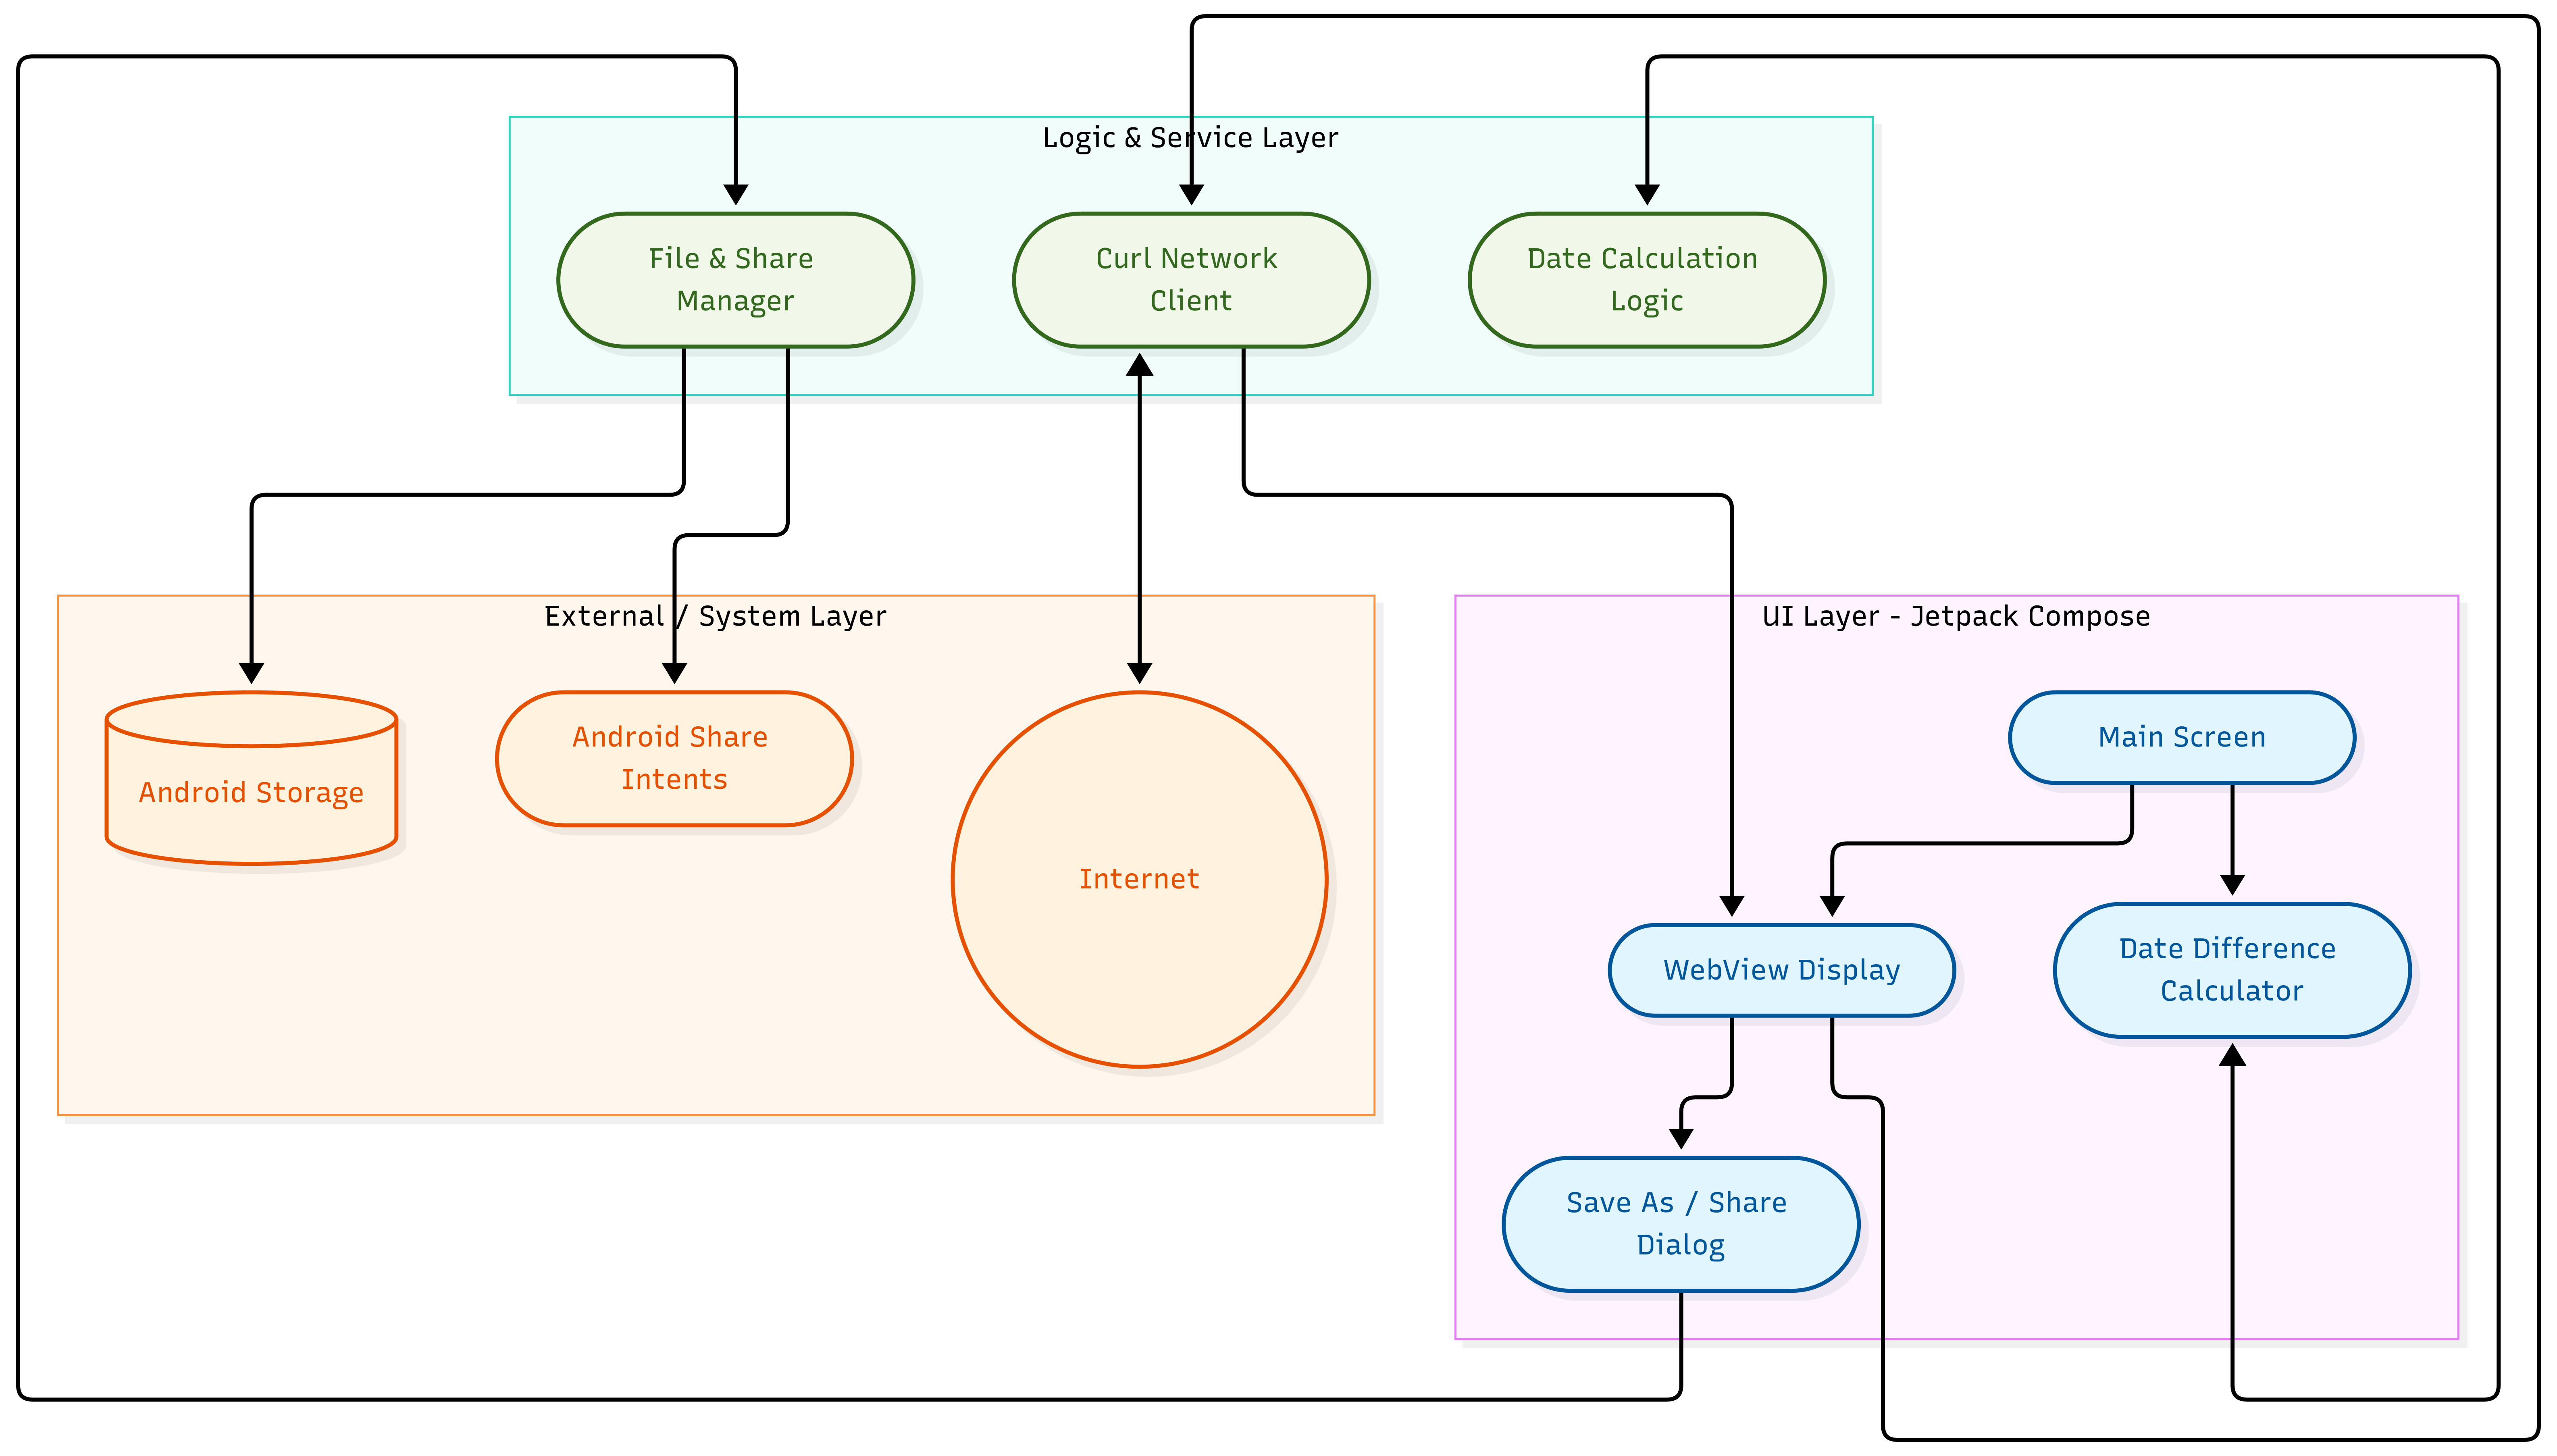
\includegraphics[width=\linewidth]{architecture-graph.png}    \caption{Application architecture graph \citep{app-graph}}
    \label{fig:app-architecture-graph}
\end{figure}

\subsection{Curl-like functionality}
The curl-like functionality of the app provides the ability for a user to easily download the source of a resource located on a publicly accessible URL without rendering it or executing it as code for HTML/CSS and JavaScript respectively. additionally, it provides a way to then easily save the source file to any location on the user's device without requiring file access permissions for the app using the \hyperref[aosp]{AOSP}-provided Storage Access Framework (SAF) system intent.
This functionality can be useful for downloading the HTML source of a website and then being able to view the source and edit it in a text editor, or to download a specific file. 

\subsubsection{Main screen}
\parbox[t]{\textwidth}{
When using the curl-like-functionality of the app, the user has a choice to choose a file type for the file they wish to download. Possible file types are: 

\begin{itemize}
    \item HTML
    \item JavaScript
    \item CSS
    \item Markdown
    \item Other (treats the source as plaintext)
\end{itemize}

Two variables are declared, one \textit{immutable} variable that declares the options itself, and one which stores the file format value, as shown in the code snippet below:
}
\begin{lstlisting}[caption={HtmlFetcherScreen}, label={lst:HtmlFectherScreen}, language=Kotlin]
fun HtmlFetcherScreen(
    modifier: Modifier = Modifier,
    onHtmlFetched: (String, String) -> Unit = { _, _ -> }
) {
    val options = listOf("HTML", "JavaScript", "CSS", "Markdown", "Other")
    var selectedOption by remember { mutableStateOf(options[0]) }
\end{lstlisting}
\parbox[t]{\textwidth}{
This  \textit{mutable} variable is then adjusted depending on the option the user chooses in the segmented button and then passed to \texttt{HtmlViewerActivity.kt}, where UI and app logic uses this variable for further processing. 

Two variables are used in order to avoid the possibility of null-pointer-exceptions (NPEs) which could trigger a crash of the app or be abused by an attacker. If it were possible to change the options themselves and not just which one is selected, an attacker could theoretically write arbitrary code into it.
This is unlikely to happen, since the app doesn't use any direct user input and doesn't even connect to the internet at all at this stage, however the author of this paper would like to emphasize the importance of following best practicies when it comes to cybersecurity and programming in general.
}
\begin{lstlisting}[caption={SegmentedButton}, label={1st:SegmentedButton}, language=Kotlin]
SegmentedButton(
    selected = selectedOption == option,
    onClick = { selectedOption = option },
    shape = SegmentedButtonDefaults.itemShape(index = index, count = options.size),
    modifier = Modifier.weight(1f)
    ) {
        Text(
            text = option,
            maxLines = 1,
            overflow = TextOverflow.Ellipsis
        )}
\end{lstlisting}
\parbox[t]{\textwidth}{
When the segmented button is drawn, the overflow logic automaically adjusts so that text is cut off without causing visual bugs like differing thickness of the segments or missing text on smaller screens while a clear indicator, that the text has been cut off is added. On larger screens, if the screenspace allows for it, the segmented button is adjusted to show the whole text. This is also true for foldables: When the device is unfolded, the segmented button automatically expands to fill the whole available screenspace until the whole text for each option is displayed. 
}

The application then sends an HTML GET request to the user-specified URL after validating that the specified URL is a valid HTTP or HTTPS request, if not, a warning is shown to the user. If the GET request succeeds before timeout, the application successfully parses the content into the \texttt{HtmlViewerActivity.kt}. This is the only time when the application connects to the internet. Should the connection time out or no resource be found on the specified location, the user will also be notified by an error message. While fetching, the app displays an indeterminate progress indicator, as recommended by Google's Material Design Expressive guidelines.\textsuperscript{\citep{lin-prog-ind}} The indeterminate indicator shows the user that it's unknown how long the fetching is expected to take, but that the application is busy handling the action.

\begin{lstlisting}[caption={URL parsing logic}, label={1st:urlParser}, language=Kotlin]
val parsedUrl = URL(normalizedUrl)
        require(parsedUrl.protocol == "http" || parsedUrl.protocol == "https") {
            "Only HTTP and HTTPS URLs are supported."
        }

        val connection = parsedUrl.openConnection() as HttpURLConnection
        try {
            connection.requestMethod = "GET"
            connection.connectTimeout = 15_000
            connection.readTimeout = 15_000
            connection.instanceFollowRedirects = true
            connection.connect()

            val responseCode = connection.responseCode
            require(responseCode in 200..299) { "HTTP request failed with status $responseCode" }

            connection.inputStream.bufferedReader().use { it.readText() }
        } finally {
            connection.disconnect()
        }
\end{lstlisting}
As seen above, the application takes HTTP error codes and automatically incorporates them into the error message shown to the user if an error occurs, making it easy to debug issues without even needing application logs via logcat, which aren't available to Android\texttrademark \textsuperscript{\citep{android-tm}} users, unless they enable Developer Options, which poses additional attack surface and a security degradation. If desired however, \citeauthor{grapheneos} users can easily see application logs via logcat in the app info section without enablind Developer Options. This is how the author of this paper debugged the application on their personal device without having to degrade its security, or needing an additional device for development purposes. 

\subsubsection{HTMLviewer screen}
The \texttt{HtmlViewerActivity.kt} uses the system-provided WebView and applies dynamic themeing based on the system-specified MDY colors, in order to simulate a native app experience while keeping the content inside the robust chromium sandbox, which is updated frequently. Thus, the application avoids requiring frequent updates and extensive vulnerability testing. As long as the system is kept up-to-date, the components of the app which might have undiscovered vulnerablities are updated with it. \citeauthor{grapheneos} users especially benefit from the additional hardening and frequent updates to the Vanadium system WebView. 
\begin{lstlisting}[caption={JavaScript and Storage is disabled}, label={lst:webviewhardening}, language=Kotlin]
settings.javaScriptEnabled = false
settings.domStorageEnabled = false
\end{lstlisting}

To display the HTML content without rendering it as code, additional HTML is injected around it. This code is static and not added to the content when the file is saved. This approach mitigates an attacker crafting a malicious website which would then run arbitrary code, although inside the robust chromium sandbox, without the user's consent. 
\begin{lstlisting}[caption={Dynamically themed, unrendered source view}, label={lst:htmlsourceview}, language=Kotlin]
private fun createSourcePage(htmlContent: String, contentType: String, colorScheme: ColorScheme): String {
    val background = colorScheme.background.toCssColor()
    val surface = colorScheme.surface.toCssColor()
    val surfaceContainer = colorScheme.surfaceContainer.toCssColor()
    val primary = colorScheme.primary.toCssColor()
    val onBackground = colorScheme.onBackground.toCssColor()
    val onSurfaceVariant = colorScheme.onSurfaceVariant.toCssColor()
    val outline = colorScheme.outline.toCssColor()
    return """
        <!DOCTYPE html>
        <html>
        <head>
            <meta name="viewport" content="width=device-width, initial-scale=1.0">
            <style>
                * { box-sizing: border-box; }
                html, body { margin: 0; padding: 0; background: $background; color: $onBackground; }
                body { padding: 20px 16px; font-family: sans-serif; }
                h1 { margin: 0 0 16px 4px; color: $onBackground; font-size: 22px; font-weight: 600; }
                .source-card { background: $surface; border: 1px solid $outline; border-radius: 20px; padding: 16px; }
                .source-label { margin-bottom: 12px; color: $primary; font-size: 13px; font-weight: 600; letter-spacing: 0.5px; }
                pre { margin: 0; padding: 16px; background: $surfaceContainer; border-radius: 12px; color: $onSurfaceVariant; white-space: pre-wrap; overflow-wrap: break-word; font-family: monospace; font-size: 13px; line-height: 1.5; }
                code { font-family: monospace; }
            </style>
        </head>
        <body>
            <h1>$contentType Source</h1>
            <div class="source-card">
                <div class="source-label">$contentType CODE</div>
                <pre><code>$htmlContent</code></pre>
            </div>
        </body>
        </html>
    """.trimIndent()
}
\end{lstlisting}
The "save as" Floating Action Button (FAB) on the \texttt{HtmlViewerActivity.kt} screen is a native Compose element, which also follows Google's Material 3 Expressive design guidelines. When pressed it presents the file extension depending on the user choice and when selected saves the file with the file extension the user specifies on the \texttt{MainActivity.kt} screen, where they select it using the segmented button before sending the HTML GET request for the resource.

\begin{lstlisting}[caption={MenuOptionItem}, label={lst:MenuOptionItem}, language=Kotlin]
MenuOptionItem(Icons.Default.Code, "Save as $contentType") {
    isExpanded = false
    onSaveAsSource()
}
\end{lstlisting}
\parbox[t]{\textwidth}{
The \texttt{\$extension} variable declares the file extension passed from the \texttt{MainActivity.kt} screen using the \texttt{option} variable. The app then calls a system intent to save a file without ever requesting file access permissions. This is possible thanks to the Storage Access Framework (SAF) intent provided by  \hyperref[aosp]{AOSP}.
}
\begin{lstlisting}[caption={saveAsSource}, label={lst:saveAsSource}, language=Kotlin]
private fun saveAsSource() {
    val extension = getExtensionForType(contentType)
    pendingSaveContent = htmlContent
    createDocumentLauncher.launch("${contentType.lowercase()}-source.$extension")
}
\end{lstlisting}
\subsection{Date difference calculator}
\parbox[t]{\textwidth}{
The date difference calculator is accessible to the user via the navigation bar or rail, depending on whether the app is used on a small or large display, and uses the system date picker, which can be switched from a calendar-like date picker or keyboard-based entry. By default, the calendar-like date picker is used, since this is the default in Google's own applications.

After the user specifies two dates, the application performs the calculation, regardless of what date is inputted first. It's entirely possible for the user to pick the first date to be far into the future, while the second date is far behind in the past. The application does not assume the first date has to be located before the second temporally. The author of this paper believes this makes it easier for the user to quickly input two dates and not have to re-do the entry if  they have mixed up the order of the dates, which is more convenient.

The date difference is then displayed in the amount of days. This calculation, even when performed for a large time period, is nearly instant and the performance overhead of opting into MTE is irrelevant.
}

\section{Source code}
\begin{wrapfigure}{r}{0.45\textwidth}
    
\includegraphics[width=0.9\linewidth]{gh-releases-qrcode.png}
    \caption{GitHub releases QR-code}
\end{wrapfigure}
The source code for the entire application is available on the GitHub repository\textsuperscript{\citep{androidtoolbox}} with an architectural graph in the readme and a copy of this paper with the \LaTeX source code. On devices running Android 15 or newer, the application can be installed from the GitHub releases page (\href{https://github.com/e227474/AndroidToolbox/releases}{e227474/AndroidToolbox/releases})\textsuperscript{\citep{androidtoolbox}},
which is also accessible via the QR code on the right. The application is licensed under the ISC license and the author of this paper highly encourages the use of its code for both commercial and non-commercial use. This paper itself, as stated in the preface, including the authors original text and images, is dedicated to the public domain under \href{https://creativecommons.org/publicdomain/zero/1.0/}{CC0 1.0 Universal}.

\subsection{GitHub}
The GitHub repository provides a detailed commit history log, showing all changes made with a timestamp. This acts as documentation for the work process of the app in its entirety. It's possible to look at an exact snapshot of the code at a given time for the entire codebase. The GitHub releases page also provides hyperlinks to compare a commit log between two releases, an apk build at the time of release and additional documentation in the form of screenshots and written details.
The author of this paper recommend users verify the signing certificate hash provided below before installing the application with a signing certificate hash viewer App like AppVerifier\textsuperscript{\citep{appverifier}}, or by inputting the signing certificate hash from below into the "expected signing certificate hash" field in Obtainium\textsuperscript{\citep{obtainium}}.

\begin{wrapfigure}[11]{l}{0.35\textwidth}
    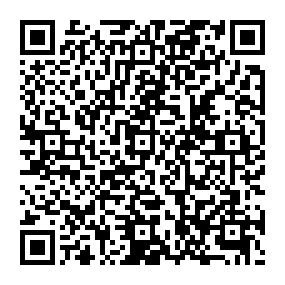
\includegraphics[width=0.9\linewidth]{signing-cert-hash.png}
    \begin{center}
        \footnotesize{signing certificate hash}
    \end{center}
\end{wrapfigure}
The QR code provided on the left can be used to easily copy the signing certificate hash to the smartphone.\textbf{ The author of this paper does not recommend installing the application if there is a singing certificate mismatch, as this can indicate that the application has been replaced with a malicious package or is corrupted.}

\begin{lstlisting}
    com.github.e227474.androidtoolbox
19:BF:76:78:C2:3D:81:47:99:9C:58:E9:58:7B:32:F6:0E:10:FC:55:C4:5C:E8:75:99:C2:8A:71:8B:55:63:79
\end{lstlisting}

For secure distribution, the author of this paper also plans to distribute this application over Accrescent\textsuperscript{\citep{accrescent}}, once the App store accepts application submissions again.\textsuperscript{\citep{accrescent-submissions-public}} This will provide an easy way for end users to download the AnddroidToolbox App with a full trust chain from the device hardware root-of-trust to the application.

\subsubsection{AI usage during development}
AI usage was kept to an absolute minimum and avoided whenever possible by the author of this paper during the planning and development of the AndroidToolbox application. All code hosted on the main branch of the Git repository of the AndroidToolbox application hosted on GitHub has been written by the author and does not include AI generated code. Until the \texttt{v0.5.0-beta} release, a small part of the code was an AI-generated snippet\textsuperscript{\citep{only-ai-code-part}}, which is not part of the \texttt{v1.0.0-stable} codebase. This code snippet was also not part of code that was active in the compiled application and only served to provide a Compose preview for the author during development, so they would be able to see the \texttt{HtmlViewer.kt} activity screen with the WebView and FAB visible for debugging and development purposes. This code snippet is provided below for transparency purposes and a permalink to the respective lines and tag is provided above. 
\begin{lstlisting}[caption={AI-generated @Compose preview snippet}, label={lst:only-ai-code-in-codebase}, language=Kotlin]
@androidx.compose.ui.tooling.preview.Preview(showBackground = true)
@Composable
private fun HtmlViewerFabMenuPreview() {
    MaterialTheme {
        Box(modifier = Modifier.size(360.dp, 640.dp)) {
            HtmlViewerFabMenu(
                onSaveAsTxt = {},
                onSaveAsHtml = {},
                onShare = {}
            )
        }
    }
}
\end{lstlisting}
The author of this paper used AI to generate this snippet because they could not figure out on their own how to provide a preview for the Floating Action Button (FAB) while keeping a blank WebView preview visible. This code snippet was not part of the actual Floating Action Button code and did not get incorporated into the application upon compilation, as stated above. Other than this code snippet, the author of this paper did not incorporate any AI-generated code directly into the application codebase, AI was only used to generate examples for the author to learn development more quickly than by pure trial and error and studying other existing codebases, which differ in scope and goals, therefore having different architectures and best practices.

\chapter{Closing remarks}
In conclusion, this paper has shown that the commonly held belief that so-called "Desktop" operating systems are inherently more secure than "Mobile" ones is not correct, or at the very least not correct in the way it is usually presented and in fact the opposite is true. As was explained throughout the paper, security is not determined by the form factor of the device(s), but by the underlying architecture, the available mitigations, and the amount of legacy complexity that has accumulated over time, resulting in technical and architectural debt. In this regard, desktop operating systems, especially those based on x86 hardware, are often in a far worse position than many people assume, because they are constrained by backwards compatibility, technical debt, and a comparatively large attack surface.

\section{Retrospection}
The author of this paper originally intended to solve these problems in a much more direct approach by creating a secure operating system from scratch, or by modifying an existing one at a very deep level. However, as was explained in the limitations section, this turned out to be unrealistic for the author due to hardware and time constraints, and a lack of proper formal computer science education and/or decades of professional software engineering experience. Because of this, the author instead chose the most realistic option available to them, which was to develop an application that extends the functionality of an existing secure platform rather than trying to replace or modify the platform itself.

This resulted in the \textit{AndroidToolbox}\textsuperscript{\citep{androidtoolbox}} application, which was designed with security in mind from the beginning and which tries to follow the same principles discussed in the theoretical part of this paper. The application is intentionally kept small, avoids unnecessary permissions where possible, and makes use of all available existing system security features instead of trying to bypass them. The project is not only a practical piece of software, which can improve daily use for a certain demographic of users, but also a demonstration of how secure software development can be approached with limited monetary and time resources.

The author believes that one of the most important aspect learned from this project is that security should not be treated as something abstract or optional: It is absolutely necessary and the result of many smaller decisions made during design, implementation, and actual development. If these decisions are made carelessly and without the proper consideration a topic as serious as cybersecurity requires, the result is unnecessary exposure to risks. If they are made carefully, even a relatively small application can be built in a way that respects the security model of the system it runs on, while also keeping maintenance burden lower. 

Finally, while the author of this paper does not claim to have solved the larger problem of insecure computing environments, they believe their project aims to show a realistic path forward for users who prioritize security over other aspects. The author also hopes that the paper can help correct some of the misconceptions discussed above and that the application may serve as a useful example and inspiration for others who want to build software with similar goals, or introduce people unfamiliar with the problems discussed in this paper to them and motiviate to strive to do the same. In accordance with this, this paper, including all of the author's original text and images, is licensed under the \href{https://creativecommons.org/publicdomain/zero/1.0/}{CC0 1.0 Universal} license.

\section{Future work}
Future work could be performed by either expanding on the work done by the author of this paper and following the same path of building on top of an already existing secure platform, or by addressing the fundamental issues of modern computing platforms and replacing the existing architecture entirely or keeping compatibility with legacy software. 
The author of this paper believes that both attempting to build upon existing architecture and creating new architecture that preserves compatibility with legacy software is a failed approach, as historically attempts to do this by well-funded organization with both monetary, time and human resources far beyond what most could dedicate to such a project have not succeeded. For the author of this paper, the conclusion is clear: The only true solution is addressing the fundamental flaws, which in turn requires fundamentally changing the architecture and re-designing everything from the ground up. 
Instead of patchwork solutions like MTE or compile flags and fuzzing, software should be inherently memory-safe and security should be based on capabilities and not permissions, since this would entirely avoid the famous confused deputy problem\textsuperscript{\citep{conf-dep}}, originally covered by Norm Hardy in his 1988 Paper \citetext{The\ Confused\ Deputy:\ (or\ why\ capabilities\ might\ have\ been\ invented)}\textsuperscript{\citep{conf-dep-original}}.
Achieving this would require abandoning decades of architecture and expending vast resources, but is the only long-term solution, as other approaches are just delaying the inevitable need to address fundamental issues and making that work harder as more technical debt is added to the computing system architecture(s). 
However, the author believes this transition can be done slowly and gradually, and remains optimistic in the efforts of corporations like Google developing microkernel projects, such as Fuchsia\textsuperscript{\citep{fuchsia}} , or non-profit organizations and individuals working on research projects like Plan9\textsuperscript{\citep{plan9}} or RedoxOS\textsuperscript{\citep{redox}} and slowly replacing legacy architectural stacks.

\bibliography{maturarbeit.bib}
\chapter*{Redlichkeitserkl\"arung}
Ich bestätige, dass ich die Arbeit selbständig durchgeführt, sämtliche Eigen- und Fremdleistungen deklariert und die verwendeten Quellen nach
den Regeln wissenschaftlichen Arbeitens nachgewiesen habe.

\today

\end{document}